%% Copernicus Publications Manuscript Preparation Template for LaTeX Submissions
%% ---------------------------------
%% This template should be used for copernicus.cls
%% The class file and some style files are bundled in the Copernicus Latex Package which can be downloaded from the different journal webpages.
%% For further assistance please contact the Copernicus Publications at: publications@copernicus.org
%% http://publications.copernicus.org


%% Please use the following documentclass and Journal Abbreviations for Discussion Papers and Final Revised Papers.


%% 2-Column Papers and Discussion Papers
\documentclass[gmd, manuscript]{copernicus}



%% Journal Abbreviations (Please use the same)

% Atmospheric Chemistry and Physics (acp)
% Advances in Geosciences (adgeo)
% Advances in Statistical Climatology, Meteorology and Oceanography (ascmo)
% Annales Geophysicae (angeo)
% ASTRA Proceedings (ap)
% Atmospheric Measurement Techniques (amt)
% Advances in Radio Science (ars)
% Advances in Science and Research (asr)
% Biogeosciences (bg)
% Climate of the Past (cp)
% Drinking Water Engineering and Science (dwes)
% Earth System Dynamics (esd)
% Earth Surface Dynamics (esurf)
% Earth System Science Data (essd)
% Fossil Record (fr)
% Geographica Helvetica (gh)
% Geoscientific Instrumentation, Methods and Data Systems (gi)
% Geoscientific Model Development (gmd)
% Geothermal Energy Science (gtes)
% Hydrology and Earth System Sciences (hess)
% History of Geo- and Space Sciences (hgss)
% Journal of Sensors and Sensor Systems (jsss)
% Mechanical Sciences (ms)
% Natural Hazards and Earth System Sciences (nhess)
% Nonlinear Processes in Geophysics (npg)
% Ocean Science (os)
% Primate Biology (pb)
% Scientific Drilling (sd)
% SOIL (soil)
% Solid Earth (se)
% The Cryosphere (tc)
% Web Ecology (we)


\begin{document}

\linenumbers

\title{An automatic and effective parameter optimization method for model tuning}


% % \Author[affil]{given_name}{surname}

\Author[1,2]{Tao}{Zhang}
\Author[3]{Lijuan}{Li}
\Author[2]{Yanluan}{Lin}
\Author[1,2]{Wei}{Xue}
\Author[1]{Haoyu}{Xu}
\Author[3]{Feng}{Xie}
\Author[1]{Xin}{Huang}

\affil[1]{Department of Computer Science and Technology, Tsinghua University, Beijing 100084}
\affil[2]{Center for Earth System Science, Ministry of Education Key Laboratory for Earth System Modeling, Tsinghua University, Beijing 100084}
\affil[3]{State Key Laboratory of Numerical Modeling for Atmospheric Sciences and Geophysical Fluid Dynamics, Institute of Atmospheric Physics, Chinese Academy of Sciences, Beijing 100029}

% %% The [] brackets identify the author with the corresponding affiliation. 1, 2, 3, etc. should be inserted.


\runningtitle{TEXT}

\runningauthor{TEXT}

\correspondence{Lijuan Li (ljli@mail.iap.ac.cn) }



% \received{}
% \pubdiscuss{} %% only important for two-stage journals
% \revised{}
% \accepted{}
% \published{}

% %% These dates will be inserted by Copernicus Publications during the typesetting process.


% \firstpage{1}

\maketitle
 

\begin{abstract}  

Physical parameterizations in General Circulation Models (GCMs), having various uncertain parameters, greatly impact model performance and model climate sensitivity.  Traditional manual and empirical tuning of these parameters is time consuming and ineffective. In this study, a ``three-step'' methodology is proposed to automatically and effectively obtain the optimum combination of some key parameters in cloud and convective parameterizations according to a comprehensive objective evaluation metrics. Results show that the optimum combination of these parameters determined using this method is able to improve model’s overall performance by 9\% in a AGCM. The method can be easily applied to other GCMs to speed up the model development process, especially regarding unavoidable comprehensive parameters tuning in model development stage.

\end{abstract}


\introduction  %% \introduction[modified heading if necessary] 

Due to current model resolution, General Circulation Models (GCMs) need to parameterize various sub-grid scale processes. However, due to the complexities involved in these processes, sub-grid scale physical processes are presented as empirical or statistical parameters in climate system models \citep{hack1994climate}. There are various empirical determined parameters, especially within cloud and convective parameterizations. Physical parameterizations aim to approximate the overall statistical outcomes of various sub-grid scale physics \citep{williams2005modelling}. Consequently, these parameterizations introduce uncertainties to climate simulations using climate system models \citep{warren1979seasonal}. In general, these new uncertain parameters are required to be calibrated or constrained when new parameterization schemes are integrated into models \citep{li2013evaluation}.


Traditionally, the uncertain parameters are manually tuned by a comprehensive comparison of model simulations with available observations. Such an approach is subjective, labor intensive, and hard to be extended \citep{hakkarainen2012closure, allen2000quantifying}. Currently, the automatic parameter calibration technique is a hot topic in uncertainty quantification of climate system models. Previous works focus on the methods of posterior distribution and probability, optimization algorithm, and data assimilation technique.


For the first class method, the confidence range of the optimization parameters is evaluated based on likelihood and Bayesian estimation. \cite{cameron1999flood} improves the forecast by the generalized likelihood uncertainty estimation (GLUE) \citep{beven1992future}, a method obtaining parameters uncertain range of a specific confidence level. The Bayesian Markov Chain Monte Carlo (MCMC) \citep{gilks2005markov} is widely used to obtain posterior probability distributions from prior knowledge. \cite{sun2013inverse} demonstrates the possibility of calibration of the hydrologic process in the Community Land Model version 4 (CLM4) \citep{lawrence2011parameterization,lawrence2007representing} with a Metropolis-Hasting algorithm, based on the MCMC approach. \cite{hararuk2014evaluation} calibrates soil carbon data in the  Community Land Model coupled with Carnegie-Ames-Stanford Approach biogeochemistry submodel (CLM-CASA) \citep{oleson2004technical,oleson2008improvements,parton1993observations}, a global land model consisting of biogeophysical and biogeochemical processes, by using an adaptive Metropolis (AM) algorithm \citep{gilks2005markov}. \cite{jackson2008error} obtains parameters posterior probability from clouds and convection physical process in the Community Atmosphere Model version 3.1 (CAM3.1) \citep{collins2004description} by multiple very fast simulated annealing (MVFSA) according a comprehensive metrics. The MVFSA method is one to two orders of magnitude faster than the Metropolis-Hasting algorithm \citep{jackson2004efficient}. However, these methods only try to get the likely area and cannot directly find the best combination of uncertain parameters with a minimum metrics value. Moreover, the posterior distribution heavily depends on the likelihood function assumed, which is usually difficult to determine for climate system model tuning problem.

Optimization algorithms can be used to search the maximum or minimum metrics value in a given parametric space. \cite{severijns2005optimizing} calibrates parameters of radiation, clouds, and convection in Speedy with downhill simplex \citep{press1992numerical, nelder1965simplex} to improve the radiation budget at the top of the atmosphere and at the surface, as well as the large scale circulation. Downhill simplex is a fast convergence algorithm when the parametric space is not high. However, it is a local optimization algorithm, not aiming to find the global optimal solution. Meanwhile, the algorithm has convergence issue when the simplex becomes ill-conditioned. \cite{yang2013uncertainty} uses  simulated stochastic approximation annealing (SSRR) \citep{liang2013simulated} to tune the parameters of the Zhang-McFarlane convection scheme to improve convection on the global circulation and climate. \cite{yang2014calibration} uses the MVFSA algorithm to calibrate a convective parameterization scheme in the Weather Research and Forecasting (WRF) model \citep{michalakes2001development}. \cite{gill2006multiobjective} calibrates the the Sacramento soil moisture accounting
(SACSMA) model \citep{Burnash1973} by multi-objective particle swarm optimization (MOPSO). SSRR requires at least ten thousands of steps to get a stable solution \citep{liang2013simulated}, and MVFSA also requires thousands of steps \citep{jackson2004efficient}. MOPSO needs dozens of individual cases in each iteration. All these global optimization algorithms lead to large number of model runs, leading to unacceptable high computation cost during model tuning. 

Data assimilation method has been well addressed for state estimation, which is also regarded as a potential solution for parameter estimation. \cite{aksoy2006ensemble} estimates the parameter uncertainty of  the NCAR/PSU Mesoscale
Model version 5 (MM5) \citep{haagenson1994penn} by the Ensemble Kalman Filter (ENKF). \cite{santiti2013simulated} presents two-stage filtering for the joint state-parameter estimation with a combination method of particle filtering (PF) and ENKF.  ENKF has the difficulty in looking for the representative samples. Moreover, same as the MOPSO method, ENKF and PF require quite a few of individual samples in each iteration, thus require more computation resources. 


Climate system model is a strongly nonlinear system, having large number of uncertain parameters. As a result, the parameter space of a climate system model is high-dimensional, multi-modal, strongly nonlinear, and not separable. The mentioned methods require long iterations for convergence. More seriously, one sample run of a climate system model might require tens or even hundreds years simulation to get the scientifically meaningful results.


To overcome these challenges, we propose a ``three-step'' strategy for calibrating the uncertain parameters in climate system models effectively and efficiently in this study. In the first step, a global sensitivity analysis method, Morris \citep{morris1991factorial, campolongo2007effective}, is chosen to eliminate the insensitive parameters by analyzing the main and interaction effects among parameters. Another global method by Sobol \citep{sobol2001global} is used to validate the results of Morris. The downhill simplex algorithm is used to solve the optimization problem because of its low computational cost and fast convergence for the low dimension parameter problem.A pre-processing of initial values is presented to perform global optimization and to resolve the issue of ill-conditioned simplex. Taking into account the complex configuration and manipulation of model tuning, an automatic workflow is designed and implemented to make the calibration process more efficient. The three-step calibration strategy is applied to Grid-point Atmospheric Model of LASG, version 2 (GAMIL2) \citep{li2013evaluation}, an AMIP/CMIP5 Atmospheric Model. The experiment results show that the model overall performance can be improved by 9\% in GAMIL2 according to the climate mean state. The method and workflow can be easily applied to other GCMs to speed up model development process, especially regarding unavoidable comprehensive parameters tuning in model development.


The remaining part of this paper is organized as follows. Section 2 introduces the automatic workflow proposed. It points out that the calibration work consists of a series of tedious processes. It is necessary to build a end-to-end automatic workflow. Section 3 describes the the details of GAMIL2, reference data, and calibration metrics. The three-step calibration strategy is presented in Section 4. Section 5 evaluates the calibration results, followed by a summary and discussion in Section 6.   


\section{The end-to-end automatic calibration workflow}

The common uncertainty quantification toolkits, such as the Problem Solving Environment for Uncertainty Analysis and Design Exploration (PSUADE) \citep{tong2005psuade}, Design Analysis Kit for Optimization and Terascale Applications (DAKOTA) \citep{eldred2007investigation}, support various calibration and uncertain analysis methods and pre-defined function interfaces.  However, To perform model tuning for today’s climate system models, there are many operations need to carry out, including parameter sampling, model configuration with different parameters, model runs during sampling and tuning, metrics diagnostics, parameter sensitivity analysis, initial values selection, and the model evaluation with optimal parameters. These common software cannot effectively organize the above model tuning process. Therefore, it is worth designing and developing a well-defined automatic end-to-end calibration workflow. 


Following the design philosophy, we implement an automatic workflow system, which supports multiple model run simultaneously, perform sample points duplication and model evaluation need to be integrated into the workflow of model tuning. More importantly, the workflow needs to be flexible and expandable to easily integrate other advanced algorithms as well as tools like PSUADE, DAKOTA. This workflow can carry flexible calibration strategies easily and efficiently, including the three-step we proposed. Users only require to specify the model to tune, the corresponding tuneable parameters of interest and their ranges, as well as the calibration method. The workflow can automatically execute any part of a calibration strategy, and produce the optimal parameters and its corresponding diagnostic results.


The architecture of the automatic workflow is in Figure 1. It consists of four components: preparation, calibration algorithm, post-processing, and task scheduler. Currently, the preparation module provides Morris and Sobol sensitivity analysis methods and other sampling methods, such as full factor, Latin Hypercube, MOAT, and Central Composite Designs. Meanwhile, this module can eliminate duplicate samples to reduce unnecessary computing loads. Moreover, the MCMC method based on adaptive Metropolis-Hastings algorithms is also provided to get the posterior distribution of uncertain parameters. The calibration algorithm module offers local and global optimization algorithms including downhill simplex, genetic algorithm, particle swarm optimization, differential evolution and simulated annealing. To make full use of the computational resource, the scheduler module schedules as many as cases to run simultaneously and coordinates the different tasks for reducing the contention and improving throughput. The post-processing module is responsible for metrics diagnostics, re-analysis and observational data management. In addition, all the intermediate metrics and their corresponding parameters are stored in a MySQL database, and can be used for posterior knowledge analysis.


\section{Model and Metrics}
\subsection{GAMIL2 description}
In this paper, the Grid-point Atmospheric Model of IAP LASG version 2 (GAMIL2) is used for evaluating our method and workflow. It takes part in the Atmospheric Model Inter-comparison Project (AMIP) of IPCC AR5, the Cloud Feedback Model Inter-comparison Project (CFMIP) and the Coupled Model Intercomparison Project Phase 5 (CMIP5) as the atmospheric component of the Flexible Global-Ocean-Atmosphere-Land System Model grid version 2 (FGOALS-g2). The horizontal resolution is 2.8$^\circ$ x 2.8$^\circ$, with 26 vertical levels. The dynamical core of GAMIL2 uses a finite difference scheme that conserves mass and effective energy \citep{wang2004design}. The moisture equation adopts the two-step shape-preserving advection scheme \citep{rucong1994two}. Compared with the pervious version GAMIL1, GAMIL2 has modifications on cloud-related processes \citep{li2013evaluation}, such as the deep convection parameterization \citep{zhang2005effects}, the convective cloud fraction \citep{xu1991evaluation}, and the cloud microphysics \citep{morrison2008new}. The tuneable parameters are selected  from deep convection, shallow convection, cloud fraction, cloud microphysical processes and boundary layer scheme, as shown in Table 1. The default parameter values come from the configuration of the standard version, which is used for AMIP/CMIP5 experiments and then is called as CNTL experiment.



\subsection{Evaluation data and metrics}
Wind, humidity, and geopotential height are derived from the European Center for Medium-Range Weather Forecasts (ECMWF) Re-Analysis (ERA) - Interim reanalysis, 1989 to 2004, and 1.5$^\circ$x1.5$^\circ$ horizontal resolution \citep{simmons2007era}. The precipitation data come from the Global Precipitation Climatology Project (GPCP), 1989 to 2004, and 2.5$^\circ$x2.5$^\circ$ horizontal resolution \citep{adler2003version}. The radiation variables come from the Earth Radiation Budget Experiment (ERBE), 1985 to 1989,  and 1.875$^\circ$x1.875$^\circ$ horizontal resolution \citep{barkstrom1984earth}. The climate mean state of the observational data are require to  remap to the grid of GAMIL2. It is noted that the duration of the simulation (2000-2004)  is inconsistent with the observational data. So we conduct a longer simulation (1989-2004) with the optimal parameters to validate the model performance with tuned parameters. The results show the consistent improvements with the short simulation.

A comprehensive metrics, including wind, temperature, humidity, geopotential height, precipitation, and radiation flux is used to quantitatively evaluate the simulation performance of overall simulation skills \citep{murphy2004quantification, gleckler2008performance, reichler2008well}. These variables are shown in Table 2. The model starts in the 2000th year and simulates 5 years. The climate mean state of the last three years is used to calculate the metrics. The calibration RMSE is defined as the spatial standard deviation (SD) of the model simulation against observations/re-analysis, as in equation (5) \citep{taylor2001summarizing,yang2013uncertainty}. To integrate the 16 output variables into an unique metrics, the SD of the default GAMIL2  simulations against observations (equation (6)) is used to scale each variable calibration RMSE. Finally, the  metrics is computed as the average value of each scaling variable, as equation (7). As a consequence, if the metrics is lower than one, the model performance gets improved.


\begin{align}
(\sigma_m^F)^2 &= \sum_{i=1}^l w(i)(x_m^F(i) - x_o^F(i))^2 \\
(\sigma_r^F)^2 &= \sum_{i=1}^l w(i)(x_r^F(i) - x_o^F(i))^2 \\
\chi^2 &= \frac{1}{N^F}\sum_{F=1}^{N^F} (\frac{\sigma_m^F}{\sigma_r^F})^2
\end{align}

$x_m^F(i)$ is the model outputs according to selected shown in the Table 2. $x_o^F(i)$ is the 
corresponding observation or reanalysis data. $x_r^F(i)$ is the reference results from CMIP5. w is 
the weight due to the different grid area. I is the total grid number in model. $N^F$ is the 
number of the chosen variables.


\section{Method}
The number of uncertain parameters in physical parameterizations of the climate system model is quite large. Most optimization algorithms, such as particle swarm optimization (PSO), downhill simplex, and simulated annealing algorithm are ineffective in high dimension problems. Iterations for convergence will increase exponentially with the parameters need to be tuned.  In addition, climate models generally need a long simulation to have meaningful results. Moreover, some components of the climate system model, such as atmosphere and ocean, require a long time to get significant results. Therefore, solving high dimension parameter tuning problem suffers from extreme calibration computational cost.  Thus, it is necessary to reduce the parameters dimension before the optimization.


Parameter tuning for a climate system model is to solve a global optimization problem in theory.  But traditional evolutionary algorithms, such as genetic algorithm \citep{goldberg1989messy}, differential evolutionary (DE) \citep{storn1995differential}, and PSO, generally require at least  thousands of iterations to get a stable global solution and need to set a population of individuals in each iteration, leading to high computational cost \citep{hegerty2009comparative,shi1999empirical}. Model tuning is always a trade-off between performance and computational cost. Therefore, it is the most important thing to get the best possible results with limited iterations as well as model runs for model tuning. Taking into account  this practical requirement, local optimal algorithms can play an important role, which have good performance with a cheap computational cost. 


In this paper, we propose an effective and efficient calibration strategy for model tuning problem with high dimension of parameter space. In the first step, the number of tuning parameters is reduced by eliminating the insensitive parameters during the optimization; In the second step, fast convergence for better solution is achieved by pre-selecting proper initial values and by using the downhill simplex method as the following optimal algorithm in the third step. 


\subsection{Sensitive parameter determination}

The Morris method \citep{morris1991factorial, campolongo2007effective} is a qualitative global sensitivity method. The advantage of this method is that not only the single parameter sensitivity can be calculated, but also the interactive sensitivity among parameters can be got at the same time. 

The sampling strategy is based on Morris’s one-step-at-a-time (MOAT) experimental design for relatively less samples required. It only needs $(n+1) \times M$ samples, where \textit{n} is the number of calibration parameters and \textit{M} is the number of trajectories, usually from 10 to 20. Considering the \textit{n} parameters $x_i (i=1,...,n)$, normalized to [0,1], the influence of each variable is defined as an elementary effect, shown as equation (1), where $\Delta$ is the step size for each parameter. The starting point of a trajectory is selected randomly and the next point is chosen by changing one unchanged parameter value at one time in a random order until getting $n+1$ samples. The mean of $|d_j|$ stands for the main effect of a single parameter, and the standard deviation presents the interactive effect among multiple parameters. Therefore, those parameters with a low mean and low standard deviation is regared as the insensitive ones for metrics and will be eliminated during following optimization step. 

\begin{align}
& d_{ij} = \frac{y(X_1,...,X_j+\Delta,...,X_N)-y(X_1,...,X_j,...,X_N)}{\Delta} \\
& \mu_j = avg(|d_{i,j}|), \sigma_j = stddev(d_{i,j}) 
\end{align}

Taking GAMIL2 as an example, tuneable parameters in Table 2 are required to perform sensitivity analysis. We perform 80 samples, and the results are shown in Figure 1. The insensitivity parameters, ke, capelmt, and c0 of shallow convection, will not be taken into consideration in the next step.


The parameter elimination step is critical for the final result of model tuning. To validate the results got by Morris, we compare the results with those with Sobol’s benchmark method \citep{sobol2001global}. It is also a quantitative method based on variance decomposition requiring more samples than the Morris, with a higher computation cost. The variance of the model output can be decomposed as equation (3), where \textit{n} is the number of parameters, and $V_i$ is the variance of the $i_{th}$ parameter, and $V_{ij}$ is the variance of the interactive effect between the  and $j_{th}$ parameters, and so on. The total sensitivity effect of $i_{th}$ parameter can be presented as equation (4), where $V_{-i}$ is the total variance except for the $x_i$ parameter. The Sobol results are shown as Figure 2.  The screened out parameters are the same ones as those of the Morris.

\begin{align}
& V = \sum_{i=1}^n V_i + \sum_{1 \leq i < j \leq n} V_{ij} + ... + V_{1,2,...,n}  \\
& S_{T_i} = 1 - \frac{V_{-i}}{V} 
\end{align}


\subsection{Optimization method and initial value selection}

We choose the downhill simplex method to tune the uncertain parameters for climate system models with relatively low computation cost. Downhill simplex searches the optimal solution by changing the shape of a simplex, which represents the optimal direction and step length. A simplex is a geometry, consisting of $N+1$ vertexes and their interconnecting edges, where \textit{N} is the number of calibration parameters screened in Section 2.1. The vertexes stand for the pair of a set of parameters and their metrics. The new vertex is determined by expanding and shrinking the vertex with the highest metrics value, leading to a new simplex \cite{press1992numerical} and \cite{nelder1965simplex}.


Mathematically, the downhill simplex method is a local optimization algorithm. Its convergence performance strongly depends on the quality of the initial values. For better initial values, we need to find the parameter combinations with the smaller metrics around the final solution. Moreover, we have to complete the searching as fast as possible for minimal overhead. For these two objectives, a hierarchical sampling based on the full factor sample method is used. The method uses a longer distance to find the candidate regions for the optimal solution first followed by a second round sampling using a smaller distance to reduce the interested region. The simple sampling method is easy to implement and has lower overhead compared to other complex adaptive sampling methods. 


At the same time, inappropriate initial values may lead to ill-conditioned simplex geometry, which can be found in model tuning. One issue we meet is that some parameters keep the same value in the initial values. As a result, these parameters are invariant during the optimization by using the downhill simplex method and this leads to poor performance of optimization. Consequently, simplex checking is conducted to keep as many as different parameters values during looking for initial values. Well-conditioned simplex geometry will increase the parameter freedom for optimization and get better convergence. This procedure is presented as the initial values pre-processing of the downhill simplex algorithm.


It is noted that samples for looking for initial values might be the same ones in dimension reduction step. In this case, one model run can be used in the two steps, saving computational resource.


\subsection{Evaluate the tuning performance}

We compare the tuning effectiveness and efficiency with global and local optimization methods in Table 3. For the global algorithms, the population size of DE and PSO is set to twelve. The parameters required to calibrate are shown in Table 1.   The effectiveness is evaluated by the final optimal solution, and the efficiency is evaluated by the core hours consumed, which are computed as $N_{step} \times N_{size} \times 30 \times 6$, where $N_{step}$ is the number of iterations and $N_{size}$ is the population size. Every GAMIL2 experiment runs with thirty cores, taking six hours for five–year simulation. 


In table 3, PSO gets the best solution. But this global method spends more computational cost than the local downhill simplex method. Taking into account the bad effectiveness of downhill simplex, we present two optimal strategies, the proposed three-step in this paper, and the ``two-step'' method only having the initial values pre-processing and downhill simplex method (Tao Zhang et al., Quantification and optimization of parameter uncertainty in the Grid-point Atmospheric Model GAMIL2, manuscript in review, 2014). The downhill simplex in the three-step tunes the sensitivity parameters described in section 2.1. The initial values pre-processing requires extra 25 sampling points, and the parameters sensitivity analysis with Morris requires 80 sampling points. The two-step gets a better solution than the ``one-step'' downhill simple. It indicates pre-selecting the proper initial values can remarkablely improve the calibration performance. Although the ``two-step'' method has the best efficiency, while the solution is worse than the ``three-step'' method. Meanwhile, the computational cost of all strategies based on the local algorithm are better than the global method. With the results in Table 3 and Table 4, we can conclude that our proposed three-step method can get the best trade-off between accuracy and computation cost.   




\section{The mechanism analysis}

Figure 4 exhibits the Taylor diagram of the 16 variables for three years of the climate mean state from 2002 to 2004.  No variable of EXP becomes much less than CNTL. Instead,  zonal wind at 850 hPa (U850),  zonal wind at 200 hPa (U200), meridional wind at 850 hPa (V850), meridional wind at 200 hPa (V200), and specific humidity at 400 hPa (Q400) have been improved a lot. Figure 5 shows the metrics of each variable with the global, tropic, and northern/southern middle and high latitudes (NMHL/SMHL). Most variables of the global area are improved compared with CNTL. Specific humidity at 400 hPa (Q400) is the most improved. Two variables, meridional wind at 200 hPa (V200) and clearsky short wave net flux at TOA (FSNTOAC) keep the same magnitude. Temperature  at 850 hPa and 200 hPa are worse than CNTL. From the spatial distribution perspective, the SMHL contributes the most improvement.


Figure 5 presents the improvement of all the radiation variables. This could be attributed to  specific humidity and cloud improvement in the middle and upper troposphere. The EXP consumes the more water vapor and achieves a the better simulation than CNTL above 700 hPa, shown in Figure 6. The decrease in the atmospheric water vapor reduces the greenhouse effect. Therefore, it emits more outgoing long-wave radiation with a clear sky, reducing the negative bias of clear sky long wave upward flux at TOA (FLUTC), as shown in Figure 8(a). 


Compared with CNTL, middle and high cloud significantly increase, as a result of the reducing rhminh parameter, shown in Figure 7. Consequently, it enhances the blocking effect on the long wave upward flux at TOA (FLUT), reducing the FLUT in 30$^\circ$/60$^\circ$ of the southern and northern hemisphere, shown in Figure 8(b). Taking into account the long wave cloud forcing (LWCF) computed as $FLUTC - FLUT$, the improvement of FLUTC in the tropics  makes up for the increasing bias of FLUT. Therefore, the LWCF in tropics stays the same as CNTL. But the LWCF in the middle and high latitudes is improved due to the improvement of FLUT in this area, as shown in Figure 8(c).


\conclusions  %% \conclusions[modified heading if necessary]  

In this paper, we present the ``three-step'' method for tuning uncertain physical parameters in climate system models effectively and efficiently, including dimension reducation step, step of pre-processing initial values, and optimization step with the downhil simplex method. To improve the convergence and the solution of downhill simplex, an initial values pre-processing algorithm is presented to evaluate the likely area of the optimal solution quickly and to resolve the issue of ill-conditioned simplex. Moreover, an automatic parameters calibration workflow is further designed and implemented to further enhance operation efficiency and to support multi uncertainty quantification analysis and calibration strategy. The experiment results over AGCM model of GAMIL2 show the ``three-step'' outperforms the PSO and DE in both effectiveness and efficiency and has a good trade-off between accuracy and computation cost compared with ``two-step'' methods and downhill simplex method. The optimal results of the ``three-step'' method demonstrate most of the variables are improved compared with the CNTL experiment, especially for the radiation related variables. The mechanism analysis demonstrates that the reduced simulation errors of water  vapor have a direct effect on FLUT, and via cloud fraction indirectly influences FLUTC. The  LWCF is improved following the improved FLUT and FLUTC.

In the future, we plan to evaluate the computation-cheap surrogate model, further reducing the computational cost for calibrating the climate system model. In addition, more analysis need to be conducted to well understand the model behavior.
 
% \appendix
% \section{}    %% Appendix A

% \subsection{}                               %% Appendix A1, A2, etc.




% \begin{acknowledgements}
% TEXT
% \end{acknowledgements}


% %% REFERENCES

% %% The reference list is compiled as follows:

% %\begin{thebibliography}{}

% %\bibitem[AUTHOR(YEAR)]{LABEL}
% %REFERENCE 1
% %
% %\bibitem[AUTHOR(YEAR)]{LABEL}
% %REFERENCE 2
% %
% %\end{thebibliography}

% %% Since the Copernicus LaTeX package includes the BibTeX style file copernicus.bst,
% %% authors experienced with BibTeX only have to include the following two lines:
% %%
\bibliographystyle{copernicus}
\bibliography{uq}
%%
%% URLs and DOIs can be entered in your BibTeX file as:
%%
%% URL = {http://www.xyz.org/~jones/idx_g.htm}
%% DOI = {10.5194/xyz}


%% LITERATURE CITATIONS
%%
%% command                        & example result
%% \citet{jones90}|               & Jones et al. (1990)
%% \citep{jones90}|               & (Jones et al., 1990)
%% \citep{jones90,jones93}|       & (Jones et al., 1990, 1993)
%% \citep[p.~32]{jones90}|        & (Jones et al., 1990, p.~32)
%% \citep[e.g.,][]{jones90}|      & (e.g., Jones et al., 1990)
%% \citep[e.g.,][p.~32]{jones90}| & (e.g., Jones et al., 1990, p.~32)
%% \citeauthor{jones90}|          & Jones et al.
%% \citeyear{jones90}|            & 1990

\clearpage
%% FIGURES

%% ONE-COLUMN FIGURES

%f
\begin{figure}[t]
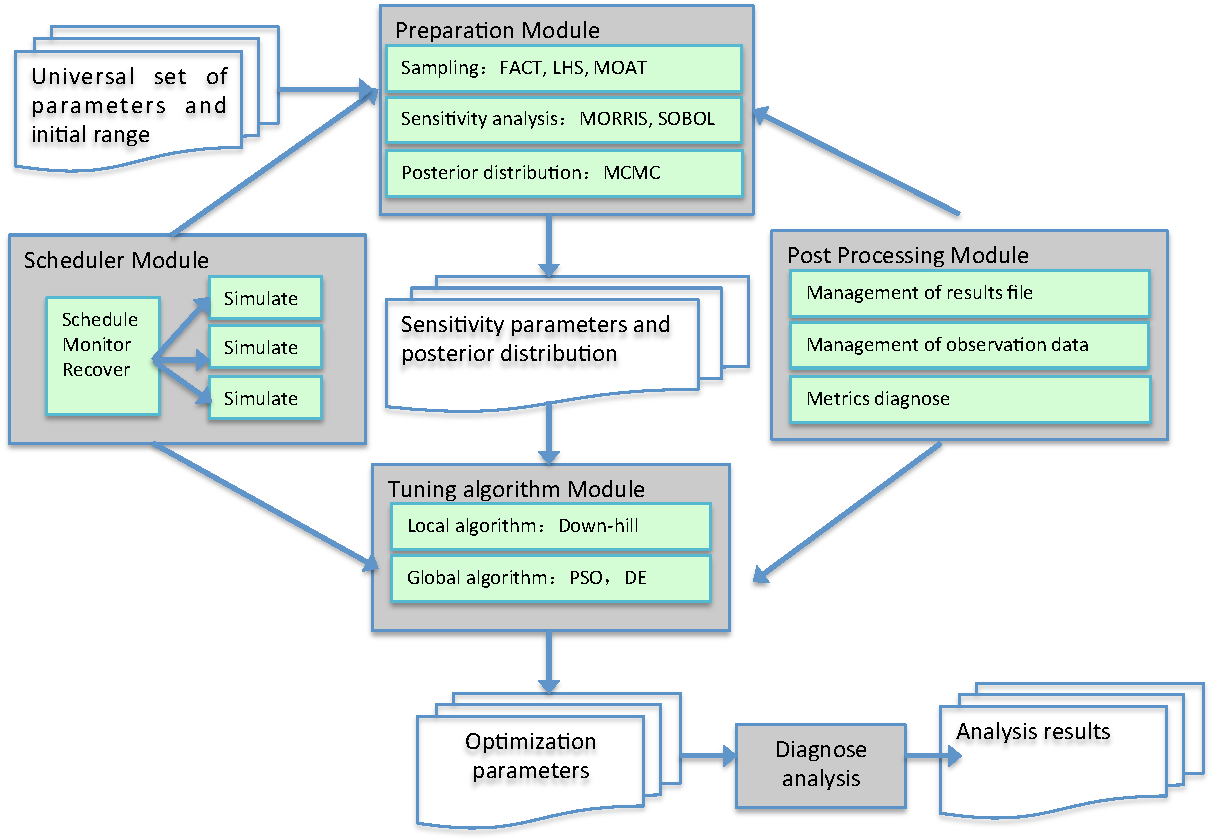
\includegraphics[width=15.3cm]{workflow}
\caption{The structure of the automatic calibration workflow.The input of the workflow is the parameters of interest and their initial value range. The
output is the optimal parameters and its corresponding diagnostic results after calibrating with a calibration strategy. The preparation module provides the parameter sensitivity analysis. The calibration algorithm module offers local and global optimization algorithms including downhill simplex, genetic algorithm, particle swarm optimization, differential evolution and simulated annealing. The scheduler module schedules as many as cases to run simultaneously and coordinates the different tasks. The post-processing module is responsible for metrics diagnostics, re-analysis and observational data management.}
\end{figure}

\begin{figure}[t]
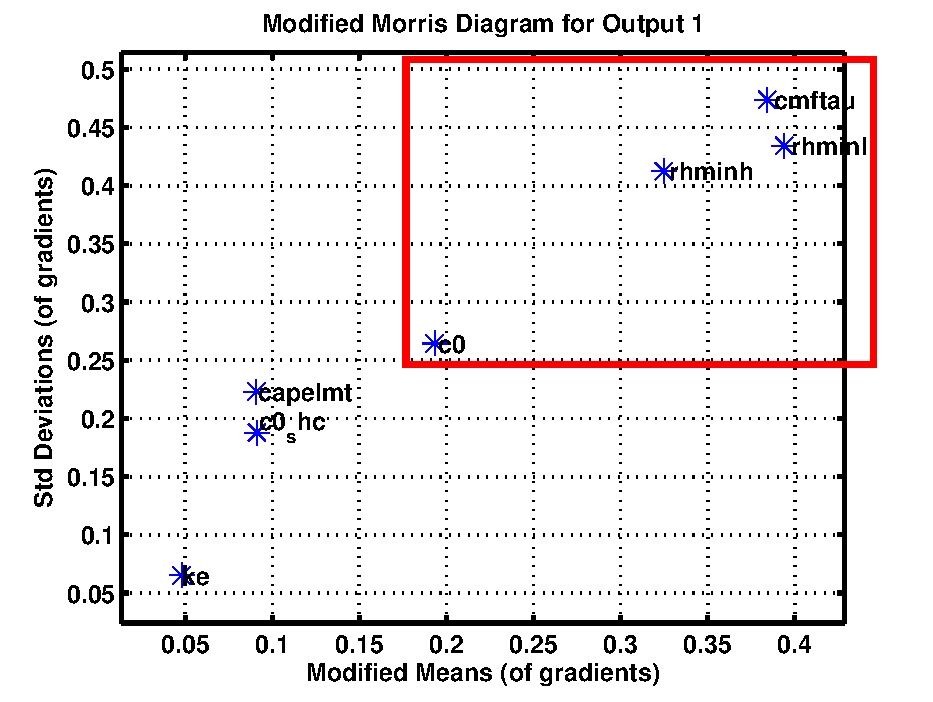
\includegraphics[width=8.3cm]{Morris}
\caption{Scatter diagram of Morris sensitivity analysis. The X-axis stands for the main effect sensitivity of single parameter. The Y-axis stands for the interactive effect among multi-parameters. Therefore, c0, rhminl, rhminh, and cmftau have high sensitivity. ke, c0\_shc, and capelmt have low sensitivity.}
\end{figure}

\begin{figure}[t]
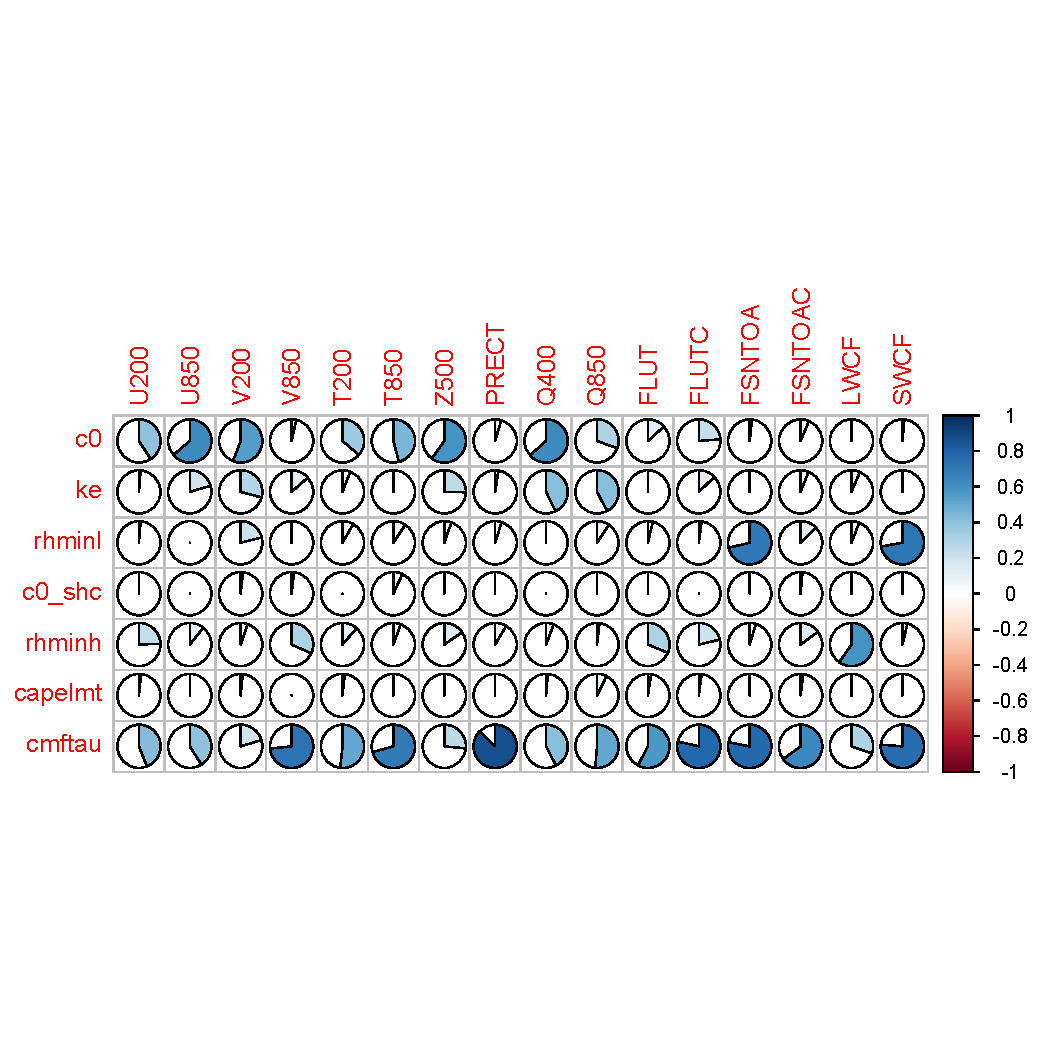
\includegraphics[width=8.3cm]{Sobol}
\caption{Sobol sensitivity results. The total sensitivity in equation (7) is presented by the size of color area. The total sensitivities of ke, c0\_shc, and capelmt are not more than 0.5 with regard to each variable. They are insensitive.}
\end{figure}

\begin{figure}[t]
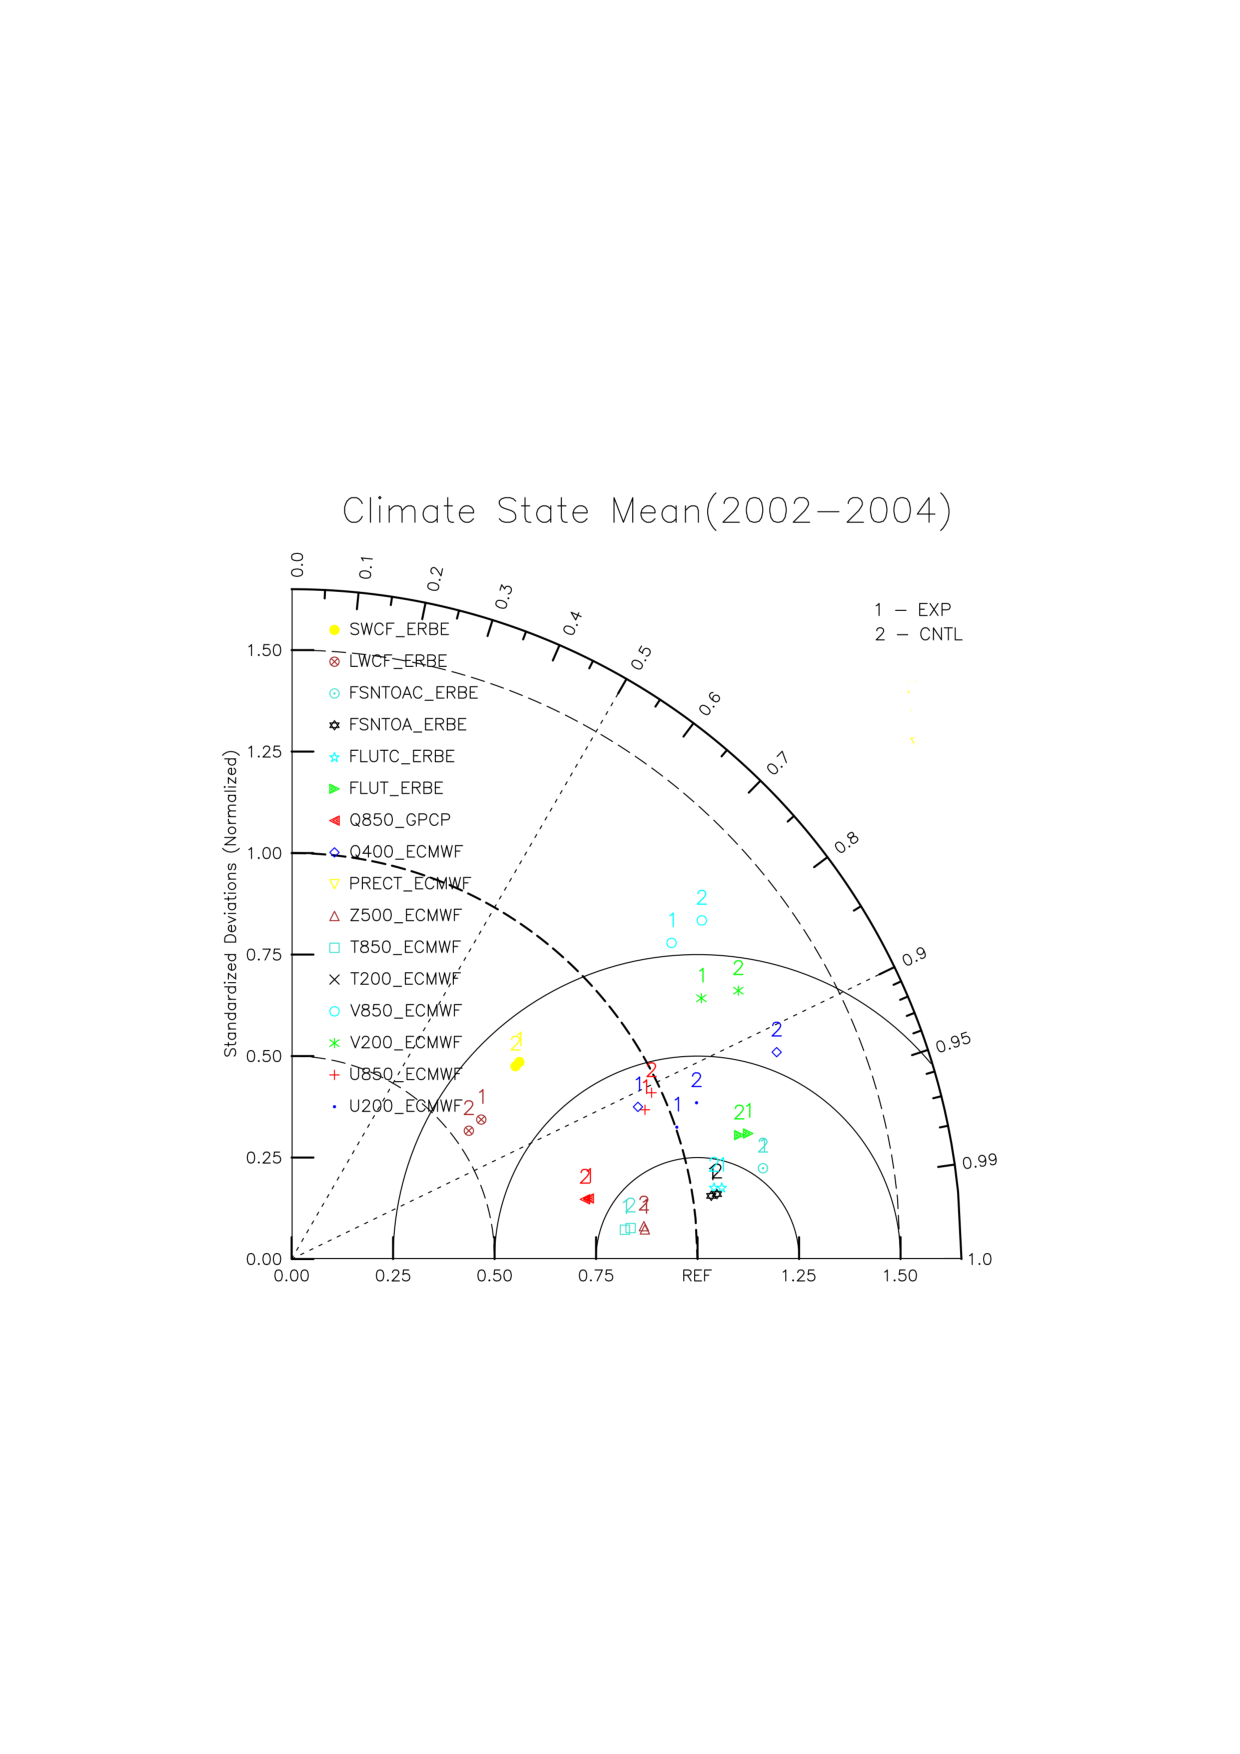
\includegraphics[width=12cm]{taylor}
\caption{Taylor diagram of the climate mean state of each variable from 2002 to 2004 of EXP and CNTL.}
\end{figure}

\begin{figure}[t]
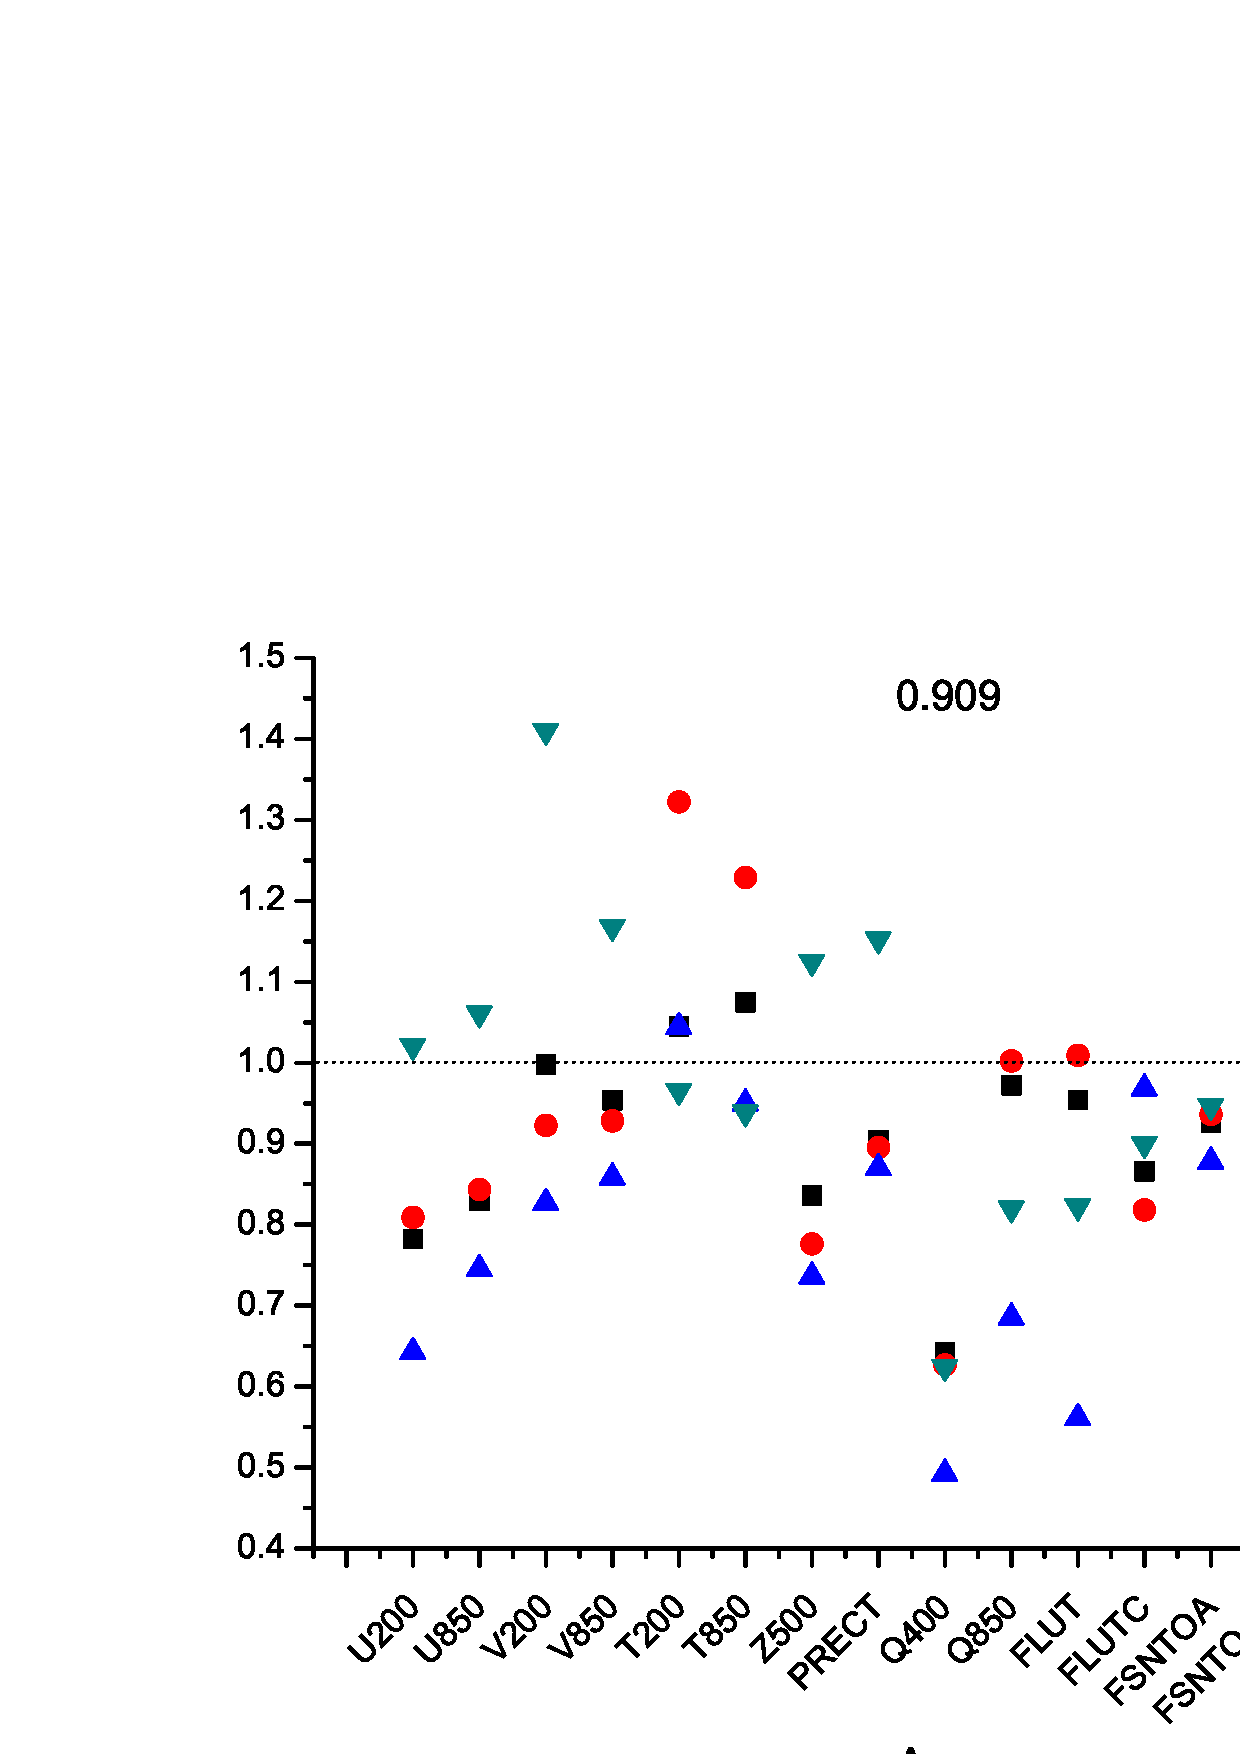
\includegraphics[width=15.3cm]{reg}
\caption{The EXP metrics of each variable with the global, tropical, and northern/southern mid- and high-latitude.}
\end{figure}

\begin{figure}[t]
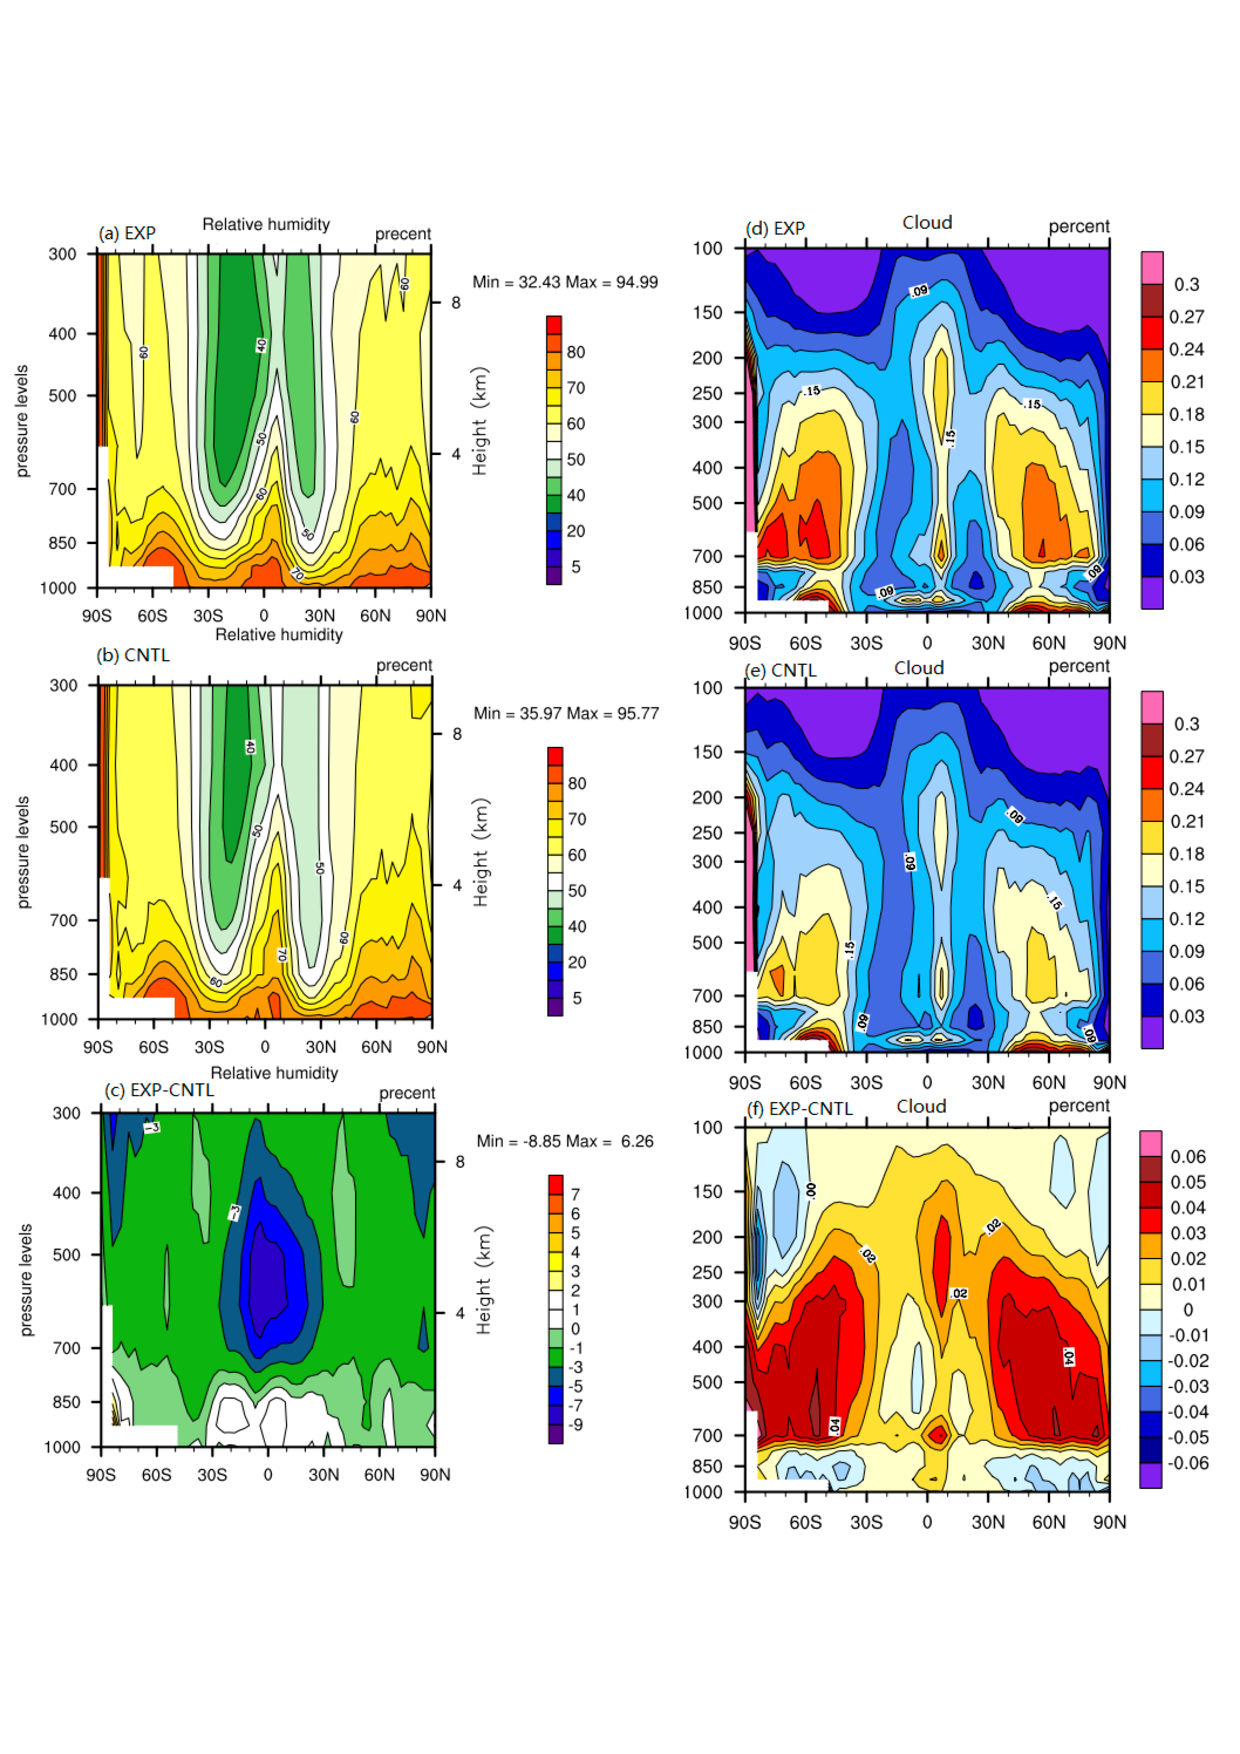
\includegraphics[width=15.3cm]{cloud-rh}
\caption{Pressure--latitude distributions of relative humidity and cloud fraction of EXP (a,d), CNTL (b,e), EXP-CNTL (c,f).}
\end{figure}

% \begin{figure}[t]
% 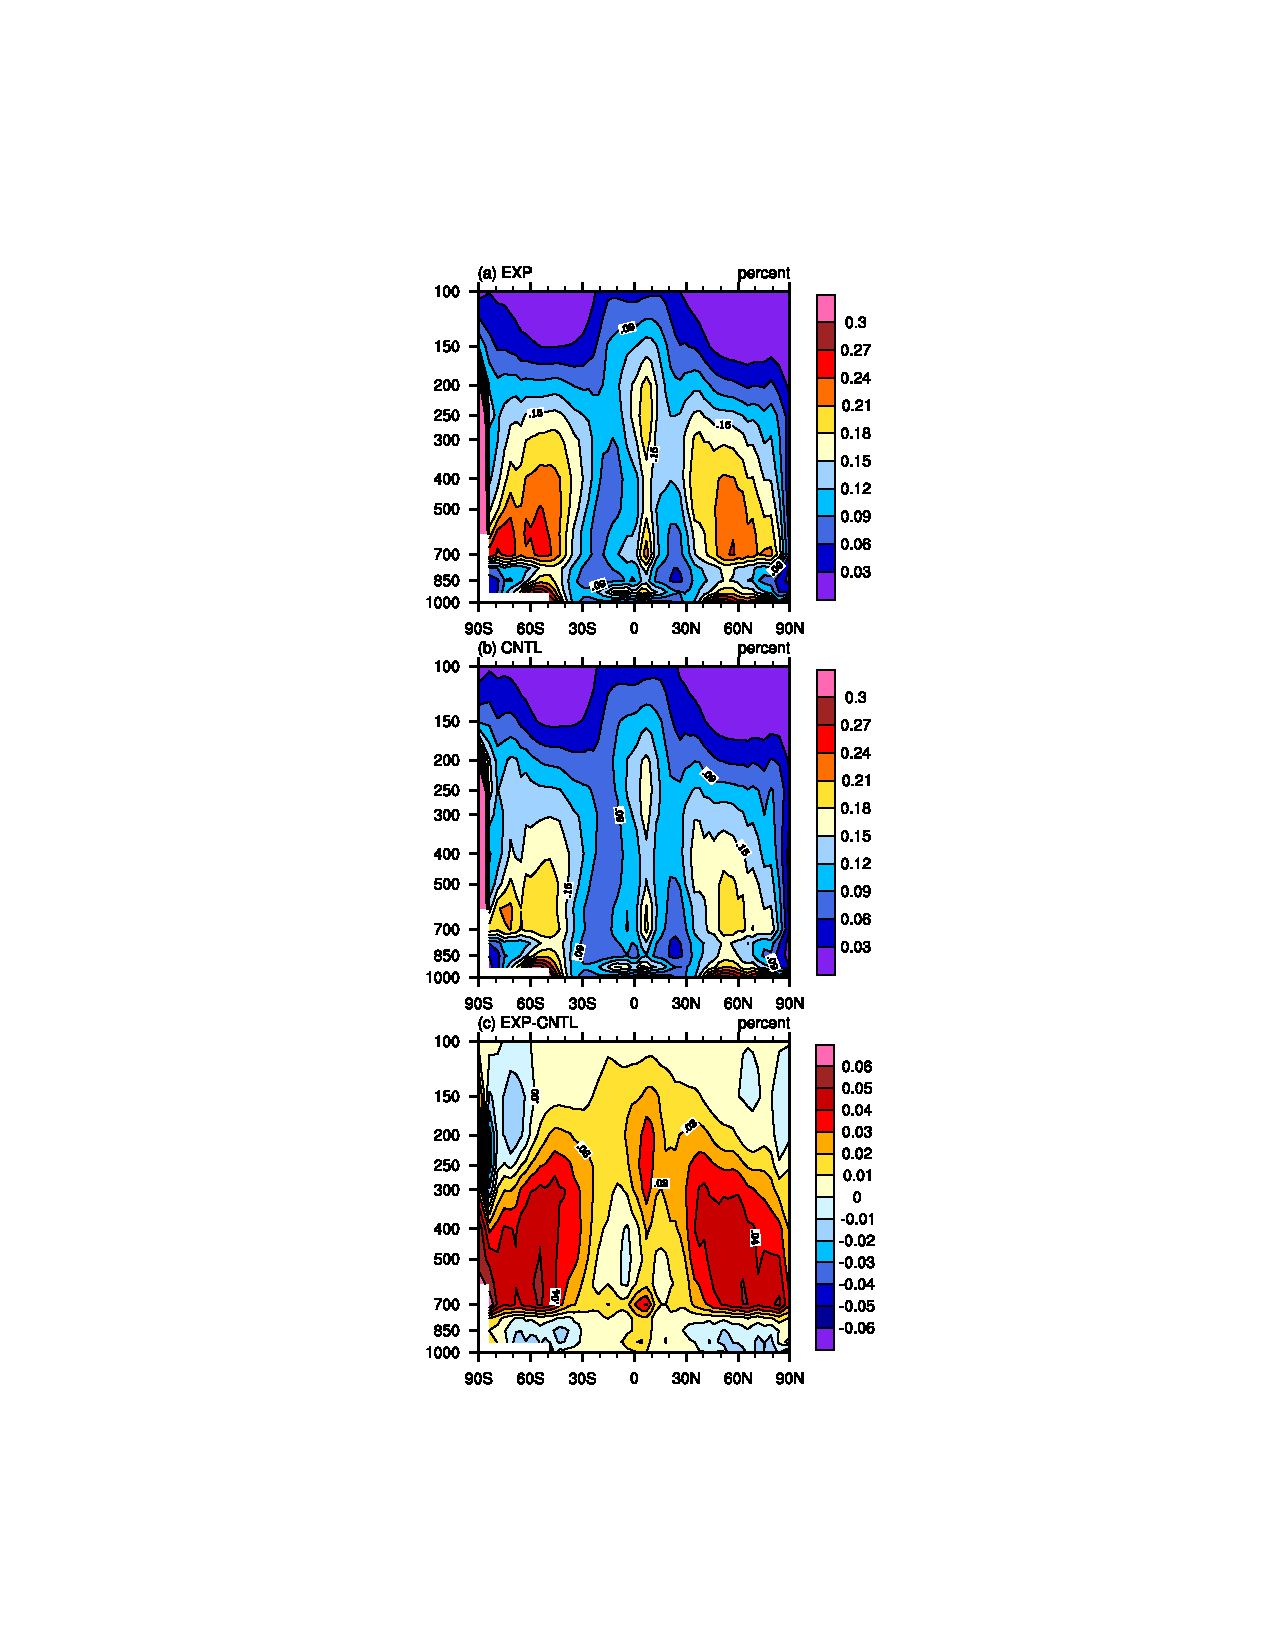
\includegraphics[width=15.3cm]{cloud}
% \caption{Pressure--latitude distributions of cloud fraction of EXP (a), CNTL (b), and EXP-CNTL (c).}
% \end{figure}

\begin{figure}[t]
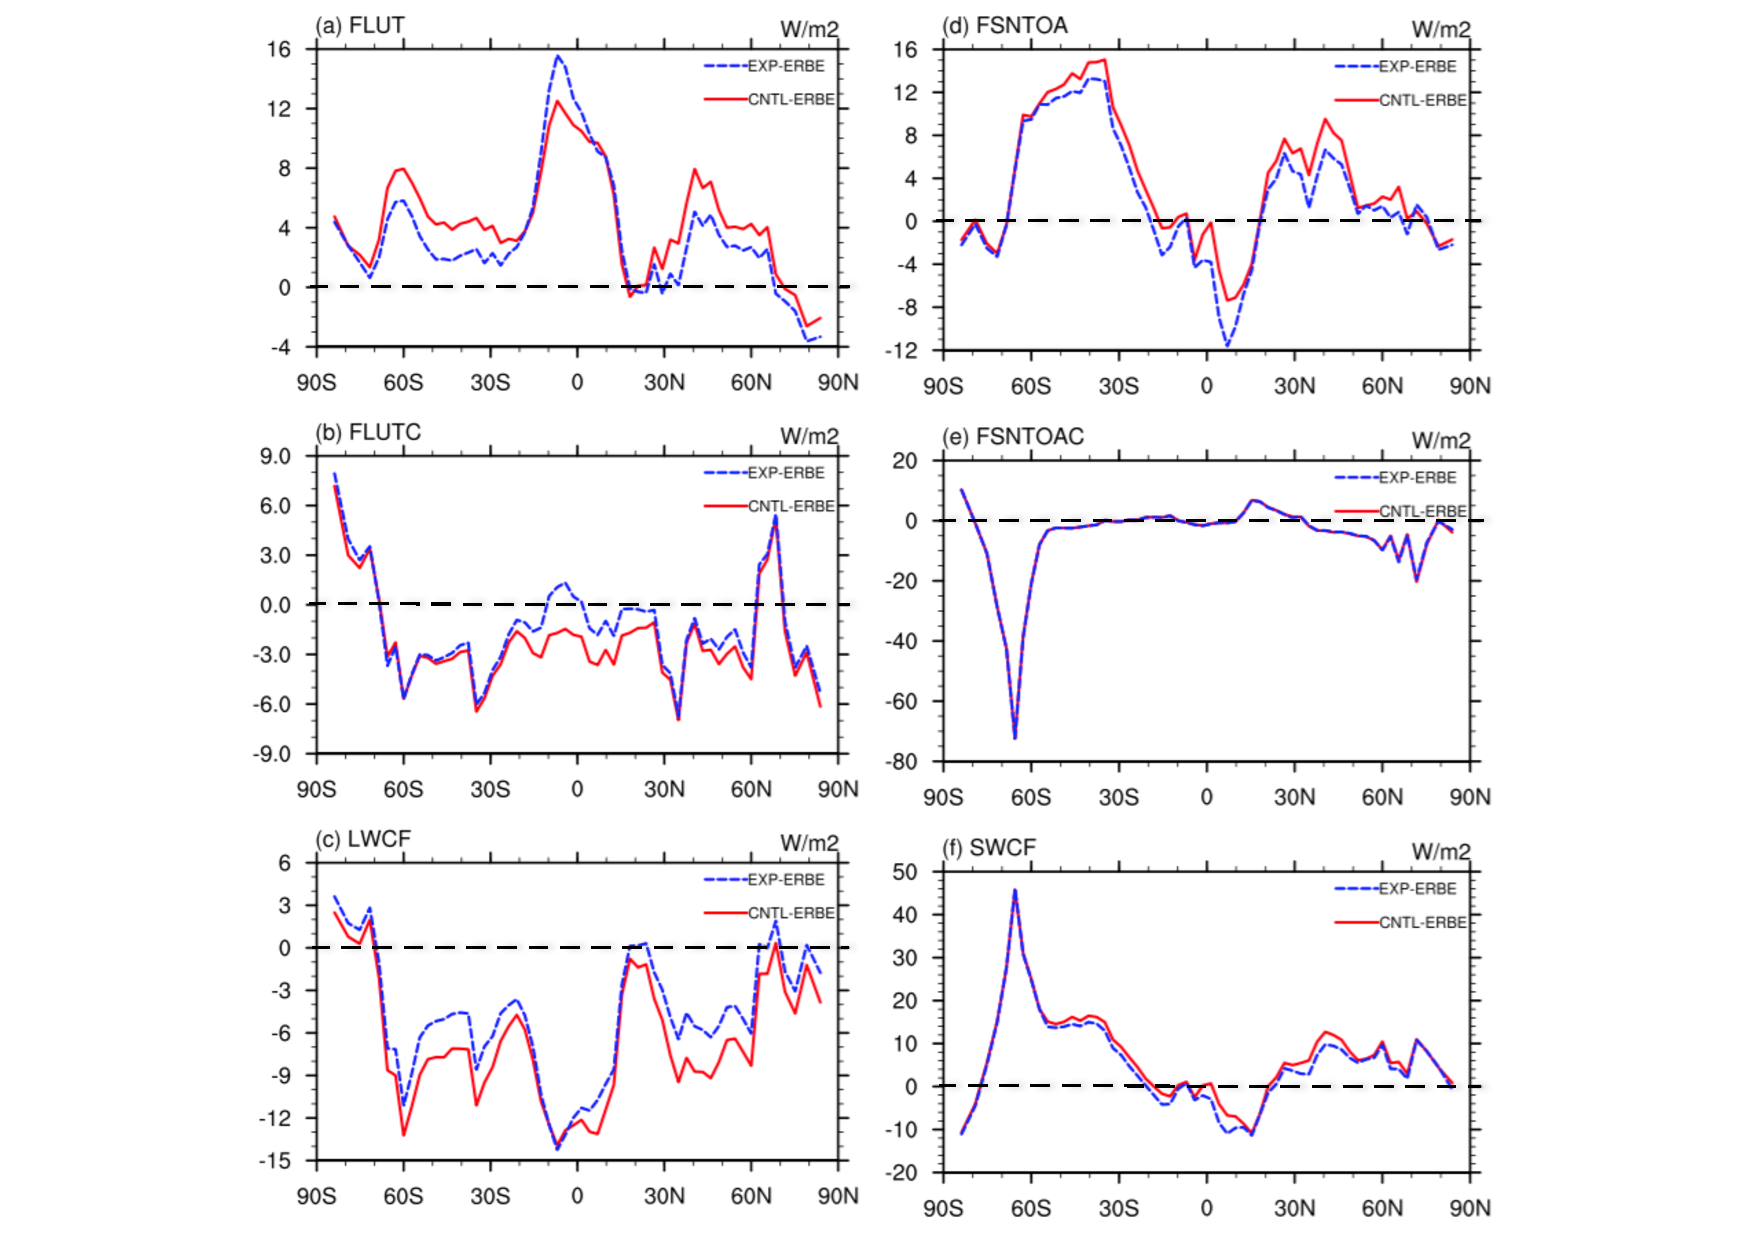
\includegraphics[width=12cm]{radiation-curve}
\caption{Meridional distributions of the annual mean difference between EXP/CNTL and observations of FLUT (a), FLUTC (b), LWCF (c), SWCF (d), FNSTOA(d), FNSTOAC(e), and SWCF(f).}
\end{figure}

\clearpage
%% TWO-COLUMN FIGURES

%f
%\begin{figure*}[t]
%\includegraphics[width=12cm]{FILE NAME}
%\caption{TEXT}
%\end{figure*}


%% TABLES
%%
%% The different columns must be seperated with a & command and should
%% end with \\ to identify the column brake.

%% ONE-COLUMN TABLE

%t

\begin{table}[t]
\caption{Initial selected uncertain parameters in GAMIL2 and their optimal values in EXP.}
\begin{tabular}{l l l c l}
\tophline
Parameter & Description & Default & Range & Optimal \\
\middlehline
c0 & rain water autoconversion coefficient for deep convection & 3.0e-4 & 1.e-4 $\sim$ 5.4e-3 & 5.427294e-4\\
ke & evaporation efficiency for deep convection & 7.5e-6 & 5e-7 $\sim$ 5e-5 & --\\
capelmt & threshold value for cape for deep convection & 80 & 20 $\sim$ 200 & --\\
rhminl & threshold RH for low clouds & 0.915 & 0.8 $\sim$ 0.95 & 0.917661 \\
rhminh & threshold RH for high clouds & 0.78 & 0.6 $\sim$ 0.9 & 0.6289215\\
c0\_shc & rain water autoconversion coefficient for shallow convection & 5e-5 & 3e-5 $\sim$ 2e-4 & -- \\
cmftau & characteristic adjustment time scale of shallow cape & 7200 & 900 $\sim$ 14400 & 7198.048 \\
\bottomhline
\end{tabular}
\belowtable{} % Table Footnotes
\end{table}

\begin{table}[t]
\caption{Model output variables and evaluation data in the metrics.}
\begin{tabular}{l l l l}
\tophline
Variable & Observation & Variable & Observation \\
\middlehline
Meridional wind at 850hPa   & ECMWF & Geopotential Z at 500hPa              & ECMWF \\
Meridional wind at 200hPa   & ECMWF & Total precipitation rate              & GPCP \\
Zonal wind at 850hPa        & ECMWF & Long-wave cloud forcing                & ERBE \\
Zonal wind at 200hPa        & ECMWF & Short-wave cloud forcing               & ERBE \\
Temperature at 850hPa       & ECMWF & Long-wave upward flux at TOA          & ERBE \\
Temperature at 200hPa       & ECMWF & Clearsky long-wave upward flux at TOA & ERBE \\
Specific Humidity at 850hPa & ECMWF & Short-wave net flux at TOA            & ERBE \\
Specific Humidity at 400hPa & ECMWF & Clearsky short-wave net flux at TOA   & ERBE \\
\bottomhline
\end{tabular}
\belowtable{} % Table Footnotes
\end{table}

% \begin{table}[t]
% \caption{Fall factor samplings of parameters and metrics.}
% \begin{tabular}{l l l l l l l l l l l l}
% \tophline
% ID & c0 & rhminl & rhminh & cmftau & metrics & ID & c0 & rhminl & rhminh & cmftau & metrics \\
% \middlehline
% 1  & 3.00E-04 & 0.915 & 0.78 & 7200 & 1     & 12 & 3.00E-04 & 0.915 & 0.6   & 7200  & 1.00547 \\
% 2  & 3.04E-04 & 0.915 & 0.78 & 7200 & 1.054 & 13 & 3.00E-04 & 0.915 & 0.675 & 7200  & 1.027676\\
% 3  & 7.13E-04 & 0.915 & 0.78 & 7200 & 0.987 & 14 & 3.00E-04 & 0.915 & 0.75  & 7200  & 1.023358\\
% 4  & 1.12E-03 & 0.915 & 0.78 & 7200 & 1.04  & 15 & 3.00E-04 & 0.915 & 0.825 & 7200  & 1.028264\\
% 5  & 2.55E-03 & 0.915 & 0.78 & 7200 & 1.075 & 16 & 3.00E-04 & 0.915 & 0.9   & 7200  & 1.160479\\
% 6  & 5.00E-03 & 0.915 & 0.78 & 7200 & 1.09  & 17 & 3.00E-04 & 0.915 & 0.78  & 900   & 1.22922 \\
% 7  & 3.00E-04 & 0.8   & 0.78 & 7200 & 1.223 & 18 & 3.00E-04 & 0.915 & 0.78  & 4275  & 1.064064\\
% 8  & 3.00E-04 & 0.838 & 0.78 & 7200 & 1.054 & 19 & 3.00E-04 & 0.915 & 0.78  & 7650  & 1.004806\\
% 9  & 3.00E-04 & 0.875 & 0.78 & 7200 & 1.019 & 20 & 3.00E-04 & 0.915 & 0.78  & 11025 & 1.077167\\
% 10 & 3.00E-04 & 0.913 & 0.78 & 7200 & 1.007 & 21 & 3.00E-04 & 0.915 & 0.78  & 14400 & 1.148265\\
% 11 & 3.00E-04 & 0.95  & 0.78 & 7200 & 1.094 \\
% \bottomhline
% \end{tabular}
% \belowtable{} % Table Footnotes
% \end{table}

\begin{table}[t]
\caption{Comparison with local and global algorithms. Downhill simplex is a local method. We use ``Downhill\_1\_step'' represents it,  distinguished from some optimal strategies based on the downhill simplex. PSO and DE are the global method. Optimal solution is the final calibrating result. $N_{step}$ is the total numbers of calibrating iteration. $N_{size}$ is the size of population of the global algorithms. Core hours is computed by $N_{step} \times N_{size} \times$ numbers of process (30) $\times$ hours of 5-years simulation (6).}
\begin{tabular}{l l l l l}
\tophline
  & Optimal solution & $N_{step}$ & $N_{size}$ & Core hours \\
\middlehline
Downhill\_1\_step & 0.9585    & 80         & 1  & 14400 \\
PSO               & 0.911537  & 24         & 12 & 51840 \\
DE                & 0.942148  & 33         & 12 & 71280 \\
\bottomhline
\end{tabular}
\belowtable{} % Table Footnotes
\end{table}

\begin{table}[t]
\caption{Comparison with optimal strategies based on the downhill simplex. The initial values pre-process is applied to Downhill\_2\_steps and Downhill\_3\_steps with extra 25 samples. In the Downhill\_3\_steps, a step of parameter sensitivity process is conducted before the initial values pre-precess with extra 80 samples.}
\begin{tabular}{l l l l l}
\tophline
  & Optimal solution & $N_{step}$ & $N_{size}$ & Core hours \\
\middlehline
Downhill\_1\_step & 0.9585    & 80         & 1  & 14400 \\
Downhill\_2\_steps  & 0.9256899 & 25+34    &  1 & 10620 \\
Downhill\_3\_steps  & 0.9098545 & 80+25+50 &  1 & 27900 \\
\bottomhline
\end{tabular}
\belowtable{} % Table Footnotes
\end{table}


% \begin{table}[t]
% \caption{The optimal parameter values.}
% \begin{tabular}{l l l}
% \tophline
% Parameter & Default & Optimal \\
% \middlehline
% c0 & 3.0e-4 & 5.427294e-4\\
% rhminl &  0.915 &  0.917661 \\
% rhminh & 0.78   & 0.6289215 \\
% cmftau &  7200  & 7198.048  \\
% \bottomhline
% \end{tabular}
% \belowtable{} % Table Footnotes
% \end{table}

\clearpage
%% TWO-COLUMN TABLE

%t
%\begin{table*}[t]
%\caption{TEXT}
%\begin{tabular}{column = lcr}
%\tophline

%\middlehline

%\bottomhline
%\end{tabular}
%\belowtable{} % Table Footnotes
%\end{table*}


%% NUMBERING OF FIGURES AND TABLES
%%
%% If figures and tables must be numbered 1a, 1b, etc. the following command
%% should be inserted before the begin{} command.

%\addtocounter{figure}{-1}\renewcommand{\thefigure}{\arabic{figure}a}


%% MATHEMATICAL EXPRESSIONS

%% All papers typeset by Copernicus Publications follow the math typesetting regulations
%% given by the IUPAC Green Book (IUPAC: Quantities, Units and Symbols in Physical Chemistry,
%% 2nd Edn., Blackwell Science, available at: http://old.iupac.org/publications/books/gbook/green_book_2ed.pdf, 1993).
%%
%% Physical quantities/variables are typeset in italic font (t for time, T for Temperature)
%% Indices which are not defined are typeset in italic font (x, y, z, a, b, c)
%% Items/objects which are defined are typeset in roman font (Car A, Car B)
%% Descriptions/specifications which are defined by itself are typeset in roman font (abs, rel, ref, tot, net, ice)
%% Abbreviations from 2 letters are typeset in roman font (RH, LAI)
%% Vectors are identified in bold italic font using \vec{x}
%% Matrices are identified in bold roman font
%% Multiplication signs are typeset using the LaTeX commands \times (for vector products, grids, and exponential notations) or \cdot
%% The character * should not be applied as mutliplication sign


%% EQUATIONS

%% Single-row equation

%\begin{equation}

%\end{equation}

%% Multiline equation



%\begin{align}
%& y=2+4x_1+4x_2-x_1^2-x_2^2+2sin(2x_1)sin(2x_2) \\
%& 0.5 \leq x_1, x_2 \leq 3.5
%\end{align}


%% MATRICES

%\begin{matrix}
%x & y & z\\
%x & y & z\\
%x & y & z\\
%\end{matrix}


%% ALGORITHM

\begin{algorithm}[htb]
\caption{Preprocessing the initial values of Downhill Simplex Algorithm.} 
\label{alg:sequential-operation}
\begin{algorithmic}
%\STATE !********************************************
%\STATE !(1) Setting the initial values
%\STATE !******************************************** 
\STATE //full factor sample 
\STATE sampling\_sets=full\_factor\_sampling(parameters\_range,number\_of\_factors) 
\STATE //refine full factor sample in the sensitivity range if needed
\IF{metrics of the the adjacent same parameter sampling points >= }
\STATE sampling\_sets+=full\_factor\_sampling(adjacent\_parameter\_range,refine\_number\_of\_factors)
\ENDIF
\STATE
\STATE //Initial vertexes with parameters of the N+1 minimum metrics
\STATE N=number\_of\_parameters 
\FOR{each initial $V_i$ of N+1 vertexes}
\STATE //get the parameters of the $i_{th}$ minimum metrics
\STATE candidate\_init\_sets += min(i, sampling\_sets) 
\ENDFOR
\STATE
\STATE //make sure the initial simplex geometry is well-conditioned
\WHILE{one parameter have the same values in the N+1 sets}
\STATE j=1
\STATE remove\_parameter\_set(the parameter set with higher metrics, candidate\_init\_sets)
\STATE //get the parameters of the $N+1+j_{th}$ minimum metrics
\STATE candidate\_init\_sets += min(N+1+j, sampling\_sets)
\STATE j+=1
\ENDWHILE
\end{algorithmic}
\end{algorithm}

% \begin{algorithm}[htb]
% \caption{Downhill Simplex Algorithm} 
% \label{alg:sequential-operation}
% \begin{algorithmic}
% %\STATE !*********************************************
% %\STATE !(2) Downhill Simplex Algorithm
% %\STATE !*********************************************
% \WHILE {step=1,2..., until convergence}
% \STATE $V_h=$vertex with the highest metrics value
% \STATE $V_{l0}=$vertex with the lowest metrics value
% \STATE $V_{l1}=$vertex with the second lowest metrics value
% \STATE !***computing the center of gravity $V_g$ except for $V_h$***
% \STATE $V_g=\frac{1}{n}(\sum_{i=1}^{N+1} V_i - V_h)$ 
% \STATE !***computing the reflection vertex $V_r$ of $V_h$ based on $V_g$***
% \ENDWHILE
% \end{algorithmic}
% \end{algorithm}


%% CHEMICAL FORMULAS AND REACTIONS

%% For formulas embedded in the text, please use \chem{}

%% The reaction environment creates labels including the letter R, i.e. (R1), (R2), etc.

%\begin{reaction}
%% \rightarrow should be used for normal (one-way) chemical reactions
%% \rightleftharpoons should be used for equilibria
%% \leftrightarrow should be used for resonance structures
%\end{reaction}


%% PHYSICAL UNITS
%%
%% Please use \unit{} and apply the exponential notation

\end{document}
